\documentclass[12pt]{article}

\usepackage[utf8]{inputenc}
\usepackage{amsmath}
\usepackage{amssymb}
\usepackage{xcolor}
\usepackage{tikz}

\begin{document}
\paragraph{\Large GBI Definitionen}
\large\subparagraph{\large RegEx}
\normalsize
\begin{flushleft}
    Wissenswertes:
    \begin{itemize}
        \item Hilfssymbole $:=$\textcolor{red}{$\{|,(,),\ast,\emptyset\}$}
        \item "$\ast$ vor $\cdot$ (Konkatenation)"
        \item "$\cdot$ vor Strich "|" (Oder)
        \item $\langle R \rangle$ ist die formale Sprache ist, welche mit $R$ gebildet werden kann
        \item $\langle \emptyset \rangle = \{\}$
        \item $\langle R_1| R_2 \rangle = \langle R_1 \rangle \cup \langle R_2 \rangle$
        \item $\langle R_1 \cdot R_2 \rangle =\langle R_1 \rangle \cdot \langle R_2 \rangle$
        \item $\langle R \ast \rangle = \langle R \rangle ^\ast$
        \item Es gibt \textbf{kein} $R+$ sondern $RR\ast$ Bsp.: Statt $(ab)+ \text{ einfach } ab(ab)\ast$
    \end{itemize}
    Bsp.: \\
    $R = a|b$ dann ist:
    \begin{align*}
        \langle R \rangle = \langle a | b \rangle = \langle a \rangle \cup \langle b \rangle = \{a\} \cup \{b\} = \{a,b\}
    \end{align*}
    $R = (a|b)\ast$ dann ist:
    \begin{align*}
        \langle R \rangle = \langle (a|b)\ast \rangle = \langle a | b \rangle^\ast = \{a,b\}^\ast
    \end{align*}
    $R = (a\ast b\ast)\ast$ dann ist:
    \begin{align*}
        \langle R \rangle &= \langle (a\ast b\ast)\ast \rangle = \langle a\ast b\ast\rangle^\ast \\
        &= (\langle a\ast\rangle\langle b\ast\rangle)^\ast = (\langle a\rangle^\ast\langle b\rangle^\ast)^\ast = (\{a\}^\ast\{b\}^\ast)^\ast \\
        &= \{a,b\}^\ast
    \end{align*}
\end{flushleft}
\large\subparagraph{\large Graphen}
\normalsize
\begin{flushleft}
    \vspace{0.5cm}
    \begin{itemize}
        \item Ein gerichteter Graph ist das Paar \textcolor{red}{$G = (V,E)$}
        \begin{itemize}
            \item \textcolor{red}{Knotenmenge $V$} ist endlich und nichtleer (V für engl. vertex)
            \item \textcolor{red}{Kantenmenge $E$} $\subseteq V \times V$  (E für engl. edge)
            \begin{itemize}
                \item muss damit auch endlich sein, darf aber leer sein
            \end{itemize}
        \end{itemize}
        \item \textcolor{red}{Pfade} können über mehrer Kanten führen
        \item \textcolor{red}{$V^{(+)}:$} Menge der nichtleeren Listen von Elementen aus V
        \item Ein Pfad ist \textcolor{red}{$p=(v_0,\dots ,v_n) \in V^{(+)}$} wenn für jedes $i \in \mathbb{Z}_n$ gilt: \textcolor{red}{$(v_i,v_{i+1})\in E$}
        \item Die Länge eines Pfades ist die Anzahl der Kanten
        \item $v_n$ von $v_0$ ist erreichbar, wenn ein Pfad $p = (v_0,\dots ,v_n)$ existiert
        \item Wenn der start und endpunkt identisch sind heißt der Pfad \textcolor{red}{geschlossen}
        \item Wenn der geschlossene Pfad größer gleich 1 ist, heißt er \textcolor{red}{Zyklus}
        \item Pfad heißt \textcolor{red}{wiederholungsfrei}, wenn
        \begin{itemize}
            \item der erste bis zum vorletzten Konten verschieden sind ($v_0,\dots ,v_{n-1}$)
            \item der zweite bis zum letzten Knoten verschieden sind ($v_1,\dots ,v_n$)
            \item der erste und letzte Knoten drüfen gleich sein ($v_0$ und $v_n$)
            \item Einfach: Außer der letzte und erste darf jeder Knoten nur einmal "betreten" werden
        \end{itemize}
        \item \textcolor{red}{azyklischer Graph}: kein Teilgraph ist zyklisch
        \item Ein Graph ist \textcolor{red}{streng zusammenhängend} wenn
        \begin{itemize}
            \item zwischen jeden beliebigen zwei Knoten (Knotenpaar) aus dem Graphen ein Pfad existiert. Also jeder Punkt von jedem anderen Punkt (sich eingeschlossen) erreichbar ist. 
        \end{itemize}
        \item Ein Graph ist ein \textcolor{red}{gerichteter Baum} wenn:
        \begin{itemize}
            \item es eine \textcolor{red}{Wurzel $r \in V$} gibt, für die gilt:
            \begin{itemize}
                \item zu jedem Knoten existiert \textbf{genau} ein Pfad
                \item Wurzel ist immer \textbf{eindeutig}
            \end{itemize}
        \end{itemize}
        \item Der \textcolor{red}{Eingangsgrad} eines Knoten ist die Anzahl aller Kanten die zu dem Knoten hinführen
        \item Der \textcolor{red}{Ausgangsgrad} eines Knoten ist die Anzahl aller Kanten die von den Knoten wegführen
        \item Der \textcolor{red}{Grad} eines Knoten ist die Anzahl der Kanten des Knotens (Also Ausgangsgrad + Eingangsgrad)
        \item Knoten eines Baumes werden \textcolor{red}{Blätter} genannt, wenn Sie das Ende des Baumes sind, also Ausgangsgrad = 0
        \item \textcolor{red}{innere Knoten} sind dann alle mit Ausgangsgrad $>$ 0
        \item $E^n$ ist ein Pfad der länge $n$. Bsp.: $E^2$ ist ein Pfad der Länge 2
        \item $(x,y) \in E^2 \Leftrightarrow$ es existiert ein Pfad der Länge 2 von $x$ nach $y$
        \item Ein ungerichteter Graph hat einfach nur Kanten und keine "Richtungs" Pfeile
        \item Knotengrad für ungerichtete Graphen: man zählt alle "Kantenenden"
    \end{itemize}
    \vspace{1cm}
    Beispiel: \linebreak
    \linebreak
    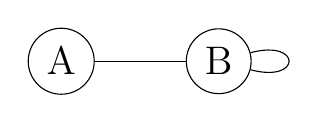
\begin{tikzpicture}[-,auto,node distance=2cm,main node/.style={circle,draw,font=\Large}]
        \tikzset{every loop/.style={}}
        \node[main node] (1) {A};
        \node[main node] (2) [right of=1] {B};
        \path
            (1) edge (2)
            (2) edge[loop right] (2);
    \end{tikzpicture} \linebreak \linebreak
    $d(B) = 3$
\end{flushleft}
\end{document}